See Figs. \ref{eq:solutions/4/3/5/fig0}, \ref{eq:solutions/4/3/5/fig1} and Table \ref{eq:solutions/4/3/5/table}



\begin{figure}[h!]
\centering
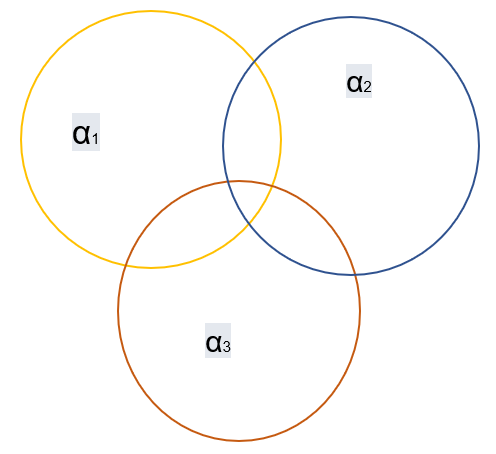
\includegraphics[width=\columnwidth]{solutions/4/3/5/index_set.png}
\caption{Index set containing $\alpha$}
\label{eq:solutions/4/3/5/fig0}
\end{figure}
%\pagebreak
\begin{figure}[h!]
\centering
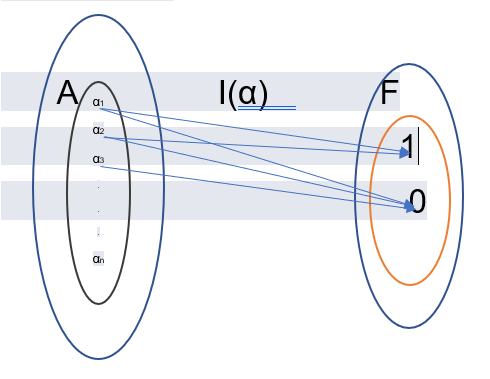
\includegraphics[width=\columnwidth]{solutions/4/3/5/ideal.png}
\caption{ideal containing $I_{\alpha}$ }
\label{eq:solutions/4/3/5/fig1}
\end{figure}

\begin{table}[h!]
\begin{center}
\begin{tabular}{|c|c|}
\hline
& \\
Given & $F$ is a field\\
%& $V(S,F)$ is a linear functional\\
%& such that\\
%& $W$ be $n$-dim subspace of $V(S,F)$.\\
%& \\
%& Also, \quad $\delta_{ij} = \begin{cases}1 \quad i=j\\ 0 \quad i \neq j \end{cases}$\\
& \\
\hline
& \\
To prove & I=$\bigcap_{\alpha \in A} I_{\alpha}$ is an ideal\\
%& \\
%& where $x_1, x_2, \dots, x_n \in S$\\
%& and $f_1,f_2,\dots,f_n \in W$\\
& \\
\hline
& \\
Proof & Let A be an index set and\\
& \\
& $I_{\alpha}$ be an in F[x] for each $\alpha \in $ A\\
& \\
&Obviously I is the subspace \\
&\\
&since $I_{\alpha}$ is a subspace of F[x]\\
&\\
& and arbitrary intersection of subspace \\
&\\
&is also a subspace. \\
&\\
& Let g\brak{x} $\in$ F[x] and f\brak{x} $\in$ I\\
&\\
& Since f\brak{x} $\in$ I\\
&\\
&and $I_\alpha$ is an ideal follows that\\
&\\
& f\brak{x} g\brak{x} $\in I_{\alpha}$ $\forall \alpha  \in A $\\
&\\
& Thus f\brak{x} g\brak{x} $\in$ I.\\
& \\
\hline
\end{tabular}
\end{center}
\caption{}
\label{eq:solutions/4/3/5/table}
\end{table}
